\section{Results}\label{sec:results}
%Results
%Show effect of colorspaces, blur, annealed mean
%Compare results of architectures (images, error plot, feature maps)
\begin{figure}[h]
	\centering
	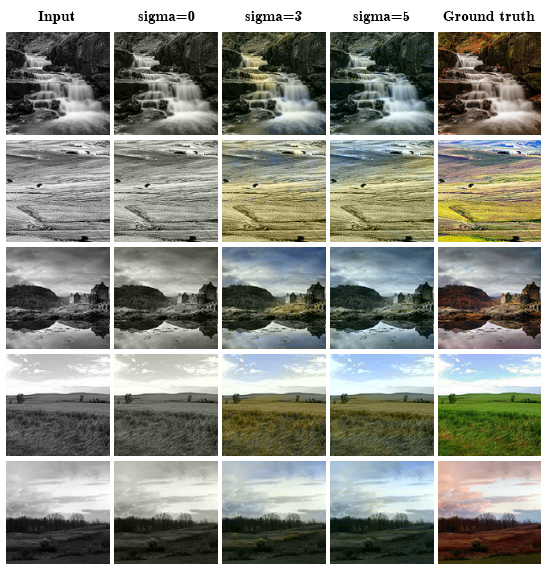
\includegraphics[width=0.6\textwidth]{blur}
	\caption{Blur}
	\label{fig:blur}
\end{figure}

\begin{figure}[h]
	\centering
	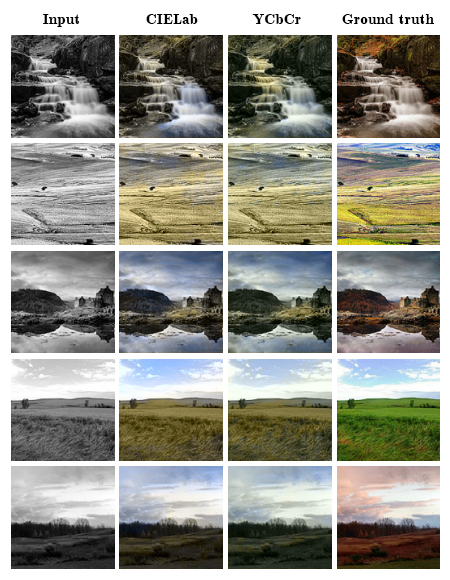
\includegraphics[width=0.6\textwidth]{YCbCr_vs_CIELab}
	\caption{YCbCr vs CIELab}
	\label{fig:YCbCr_vs_CIELab}
\end{figure}

In section \ref{sec:method} all the different techniques and methods used resulted in a selection of five final network architectures with distinct properties. In this section the results of these networks are shown in the form of colorization attempts by the various neural networks. 

\begin{figure}[h]
	\centering
	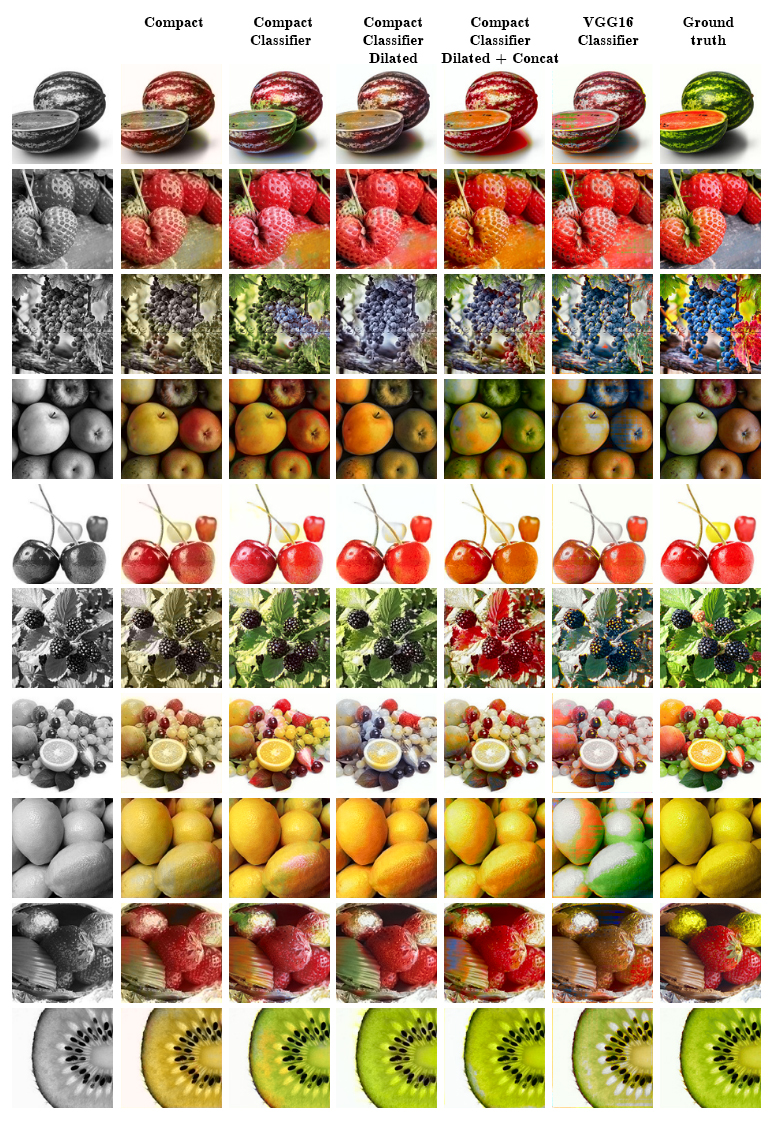
\includegraphics[width=0.9\textwidth]{set1}
	\caption{Results}
	\label{fig:results}
\end{figure}


\subsubsection{Compact}



\subsubsection{Compact classifier}


\subsubsection{Compact classifier dilated}


\subsubsection{Compact classifier dilated and concat}


\subsubsection{VGG16 compact classifier}


